\let\negmedspace\undefined
\let\negthickspace\undefined
\documentclass[journal]{IEEEtran}
\usepackage[a4paper, margin=10mm, onecolumn]{geometry}
\usepackage{lmodern} % Ensure lmodern is loaded for pdflatex
\usepackage{tfrupee} % Include tfrupee package

\setlength{\headheight}{1cm} % Set the height of the header box
\setlength{\headsep}{0mm}  % Set the distance between the header box and the top of the text

\usepackage{gvv-book}
\usepackage{gvv}
\usepackage{cite}
\usepackage{amsmath,amssymb,amsfonts,amsthm}
\usepackage{algorithmic}
\usepackage{graphicx}
\usepackage{float}
\usepackage{textcomp}
\usepackage{xcolor}
\usepackage{txfonts}
\usepackage{listings}
\usepackage{enumitem}
\usepackage{mathtools}
\usepackage{gensymb}
\usepackage{comment}
\usepackage[breaklinks=true]{hyperref}
\usepackage{tkz-euclide} 
\usepackage{listings}
% \usepackage{gvv}                                        
\def\inputGnumericTable{}                                 
\usepackage[latin1]{inputenc}                                
\usepackage{color}                                            
\usepackage{array}                                            
\usepackage{longtable}                                       
\usepackage{calc}                                             
\usepackage{multirow}                                         
\usepackage{hhline}                                           
\usepackage{ifthen}                                           
\usepackage{lscape}
\usepackage{tikz}
\usetikzlibrary{patterns}

\begin{document}

\bibliographystyle{IEEEtran}
\vspace{3cm}

\title{8.2.32}
\author{EE25BTECH11064 - Yojit Manral}

\maketitle
% \maketitle
% \newpage
% \bigskip
{\let\newpage\relax\maketitle}
\renewcommand{\thefigure}{\theenumi}
\renewcommand{\thetable}{\theenumi}
\setlength{\intextsep}{10pt} % Space between text and float

\textbf{Question:}\\
Find the conic equation that satisfies the given conditions: ends of the major axis $(0,\pm5)$, ends of the minor axis $(\pm1,0)$.

\textbf{Solution:}\\
$\rightarrow$ The equation for any conic having directrix $\vec{n}^T\vec{x}=c$ and eccentricity $e$ is given by
\begin{align}
    \vec{x}^T\vec{V}\vec{x} + 2\vec{u}^T\vec{x} + f = 0 \\
    \vec{V} = \norm{\vec{n}}^2\vec{I}-e^2\vec{n}\vec{n}^T
\end{align}
$\rightarrow$ As the major axis is along the $Y-axis$
\begin{align} \vec{n} = \vec{e_2} \implies \vec{V} = \myvec{1&0\\0&1-e^2} \end{align}
$\rightarrow$ Also, as the center of the ellipse is at origin
\begin{align} \vec{C} = 0 \implies \vec{u} = 0 \end{align}
$\rightarrow$ Let $\vec{P}$ and $\vec{Q}$ be points on the ellipse
\begin{align} \vec{P} = \myvec{1\\0} && \vec{Q} = \myvec{0\\5} \end{align}
$\rightarrow$ Then, $\vec{P}$ and $\vec{Q}$ satisfy (1)
\begin{align}
    \vec{P}^T\vec{V}\vec{P} + 2\vec{u}^T\vec{P} + f = 0& && \vec{Q}^T\vec{V}\vec{Q} + 2\vec{u}^T\vec{Q} + f = 0 \\
    \myvec{1&0}\myvec{1&0\\0&1-e^2}\myvec{1\\0} + f = 0& && \myvec{0&5}\myvec{1&0\\0&1-e^2}\myvec{0\\5} + f = 0 \\
    1 + f = 0& && 25(1-e^2) + f = 0\\
    f = -1& \implies && e^2 = 1+\frac{f}{25} = \frac{24}{25}
\end{align}
$\rightarrow$ Thus, we get the equation of the conic as
\begin{align}
    \vec{V}=\myvec{1&0\\0&1-e^2}=\myvec{1&0\\0&1/25} \text{, } \vec{u}&=0 \text{, and } f=-1\\
    \implies \vec{x}^T\myvec{1&0\\0&1/25}\vec{x} - 1 &= 0
\end{align}
\begin{figure}[h!]
   \centering
   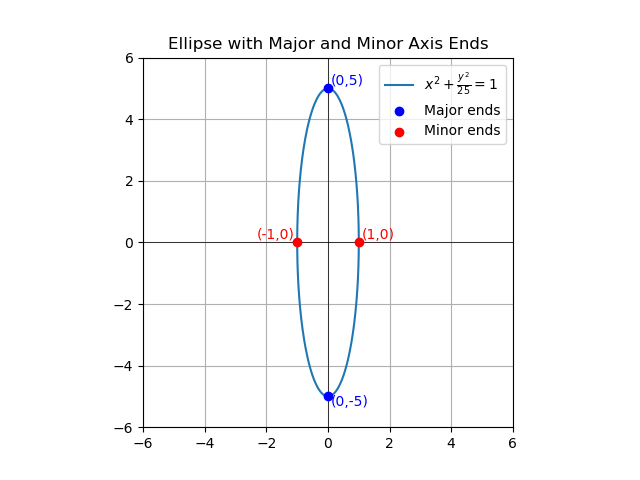
\includegraphics[width=0.65\linewidth]{figs/01.png}
   \caption{Plot of required conic}
   \label{Plot_1}
\end{figure}
\end{document}
